\documentclass{article}

\usepackage{fancyhdr}
\usepackage{extramarks}
\usepackage{amsmath}
\usepackage{amssymb}
\usepackage{enumerate}
\usepackage{graphicx}
\usepackage{braket}
\usepackage{cancel}
\usepackage{pgfplotstable}
\usepackage{listings}

\lstset{framexleftmargin=5mm, frame=shadowbox, rulesepcolor=\color{blue}}

% Useful things
\newcommand{\vcenteredinclude}[1]{\begingroup
\setbox0=\hbox{\includegraphics{#1}}%
\parbox{\wd0}{\box0}\endgroup}

%% better: (general command to vertically center horizontal material)
\newcommand*{\vcenteredhbox}[1]{\begingroup
\setbox0=\hbox{#1}\parbox{\wd0}{\box0}\endgroup}

%
% Basic Document Settings
%

\topmargin=-0.45in
\evensidemargin=0in
\oddsidemargin=0in
\textwidth=6.5in
\textheight=9.0in
\headsep=0.25in

\linespread{1.1}

\pagestyle{fancy}
\lhead{\hmwkAuthorName}
\chead{\hmwkClass\ : \hmwkTitle}
\rhead{\firstxmark}
\lfoot{\lastxmark}
\cfoot{\thepage}

\renewcommand\headrulewidth{0.4pt}
\renewcommand\footrulewidth{0.4pt}

\setlength\parindent{24pt}

%
% Create Problem Sections
%

\newcommand{\enterProblemHeader}[1]{
    \nobreak\extramarks{}{Problem \arabic{#1} continued on next page\ldots}\nobreak{}
    \nobreak\extramarks{Problem \arabic{#1} (continued)}{Problem \arabic{#1} continued on next page\ldots}\nobreak{}
}

\newcommand{\exitProblemHeader}[1]{
    \nobreak\extramarks{Problem \arabic{#1} (continued)}{Problem \arabic{#1} continued on next page\ldots}\nobreak{}
    \stepcounter{#1}
    \nobreak\extramarks{Problem \arabic{#1}}{}\nobreak{}
}

\setcounter{secnumdepth}{0}
\newcounter{partCounter}
\newcounter{homeworkProblemCounter}
\setcounter{homeworkProblemCounter}{1}
\nobreak\extramarks{Problem \arabic{homeworkProblemCounter}}{}\nobreak{}

%
% Homework Problem Environment
%
% This environment takes an optional argument. When given, it will adjust the
% problem counter. This is useful for when the problems given for your
% assignment aren't sequential. See the last 3 problems of this template for an
% example.
%
\newenvironment{homeworkProblem}[1][-1]{
    \ifnum#1>0
        \setcounter{homeworkProblemCounter}{#1}
    \fi
    \section{Problem \arabic{homeworkProblemCounter}}
    \setcounter{partCounter}{1}
    \enterProblemHeader{homeworkProblemCounter}
}{
    \exitProblemHeader{homeworkProblemCounter}
}

%
% Homework Details
%   - Title
%   - Due date
%   - Class
%   - Section/Time
%   - Instructor
%   - Author
%

\newcommand{\hmwkTitle}{Homework\ \#8}
\newcommand{\hmwkDueDate}{April 3, 2015}
\newcommand{\hmwkClass}{PHYS 5243 - Solid State Physics}
\newcommand{\hmwkClassInstructor}{Professor Sheena Murphy}
\newcommand{\hmwkAuthorName}{Chase Brown}


\begin{document}
	\begin{homeworkProblem}
		\textbf{Kittel - Introduction to Solid State Physics - Chapter 9, Problem 7: De Haas-van Alphen period of potassium}
		\\
		\begin{enumerate}[a)]
			\item Calculate the period $\Delta (\frac{1}{B})$ expected for potassium on the free electron model.
			\item What is the area in real space of the extremal orbit, for $B=10 kG=1T$ ? The same period applies to oscillations in the electrical resistivity, known as the Shubnikow-de Haas effect.
		\end{enumerate}
		\textbf{Solution}
		\\
		\begin{enumerate}[a)]
			\item Potassium is arranged in a BCC crystal lattice structure. The electron concentration in a monovalent metal with a BCC lattice structure is $n=\frac{2}{a^3}$, as there are 2 electrons within the volume of $a^3$.  Therefore, since the radius of the Fermi sphere is
				\begin{equation*}
					k_{F,K} = (3\pi^2n)^\frac{1}{3} = (\frac{6\pi^2}{a^3})^\frac{1}{3} 
				\end{equation*}
				From Table 6.1, we have $k_{F, K} = 0.75\times10^{8}cm^{-1}$.  Therefore the Fermi surface area will be $S=\pi k_{F, K}^2$, which gives the following:
				\begin{equation*}
					 \Delta (\frac{1}{B}) = \frac{2\pi\frac{e}{\hbar c}}{S} = \frac{2\pi\frac{e}{\hbar c}}{\pi k_{F, K}^2}
				\end{equation*}
				We know from the example problem in Kittel on the Fermi surface of Gold that $2\pi\frac{e}{\hbar c}=9.55\times10^7 gauss^{-1}cm^{-2}$, so using this relationship we find:
				\begin{equation*}
					 \boxed{\Delta (\frac{1}{B}) = \frac{9.55\times10^7gauss^{-1}cm^{-2}}{\pi(0.75\times10^8cm^{-1})^2}= 5.4\times10^{-9}gauss^{-1}}
				\end{equation*}
			\item In Chapter 6 of Kittel, the cyclotron frequency is defined under the \textit{Motion in Magnetic Fields} subsection as $\omega_c = \frac{eB}{mc}$.  We may use this and notice that $r = \frac{v_F}{\omega_c}$ and $v_F = \frac{\hbar k_F}{m}$.  Therefore,
				\begin{equation*}
					R = \frac{\frac{\hbar k_F}{m}}{\frac{eB}{mc}} = \frac{\hbar k_F}{eB} 
				\end{equation*}
				\begin{equation*}
					\Rightarrow R = 5\times10^{-4} cm
				\end{equation*}
				\begin{equation*}
					\Rightarrow \boxed{S = \pi (5\times10^{-4} cm)^2 = 7.8\times10^{-7}cm^2}
				\end{equation*}
		\end{enumerate}
		
	\end{homeworkProblem}
	

	\pagebreak

	\begin{homeworkProblem}
		\textbf{Fermi Surface on Hypothetical Cubic Metal}\\
		
		Consider a hypothetical monovalent monatomic simple cubic metal of lattice constant $4\AA$.  Sketch the Fermi Surface you would expect treating the valence electron as nearly free, such that the neck and belly are in the ratio of $\frac{1}{5}$.

		Suppose you able to use the de Haas-van-Alphen effect to investigate this Fermi Surface.  Describe what you would expect to see for the H field in the [100], [110] and [111] directions with H $\sim$ 1 Tesla.  Sketch the extremal orbits in each case.
\\
\\
		\textbf{Solution}\\
			
			For a Simple Cubic of lattice constant $a$ the reciprocol lattice is a simple cubic with side $\frac{2\pi}{a}$.  \\
		\\
		\textbf{B} in [100] direction:
		\\
		\centerline{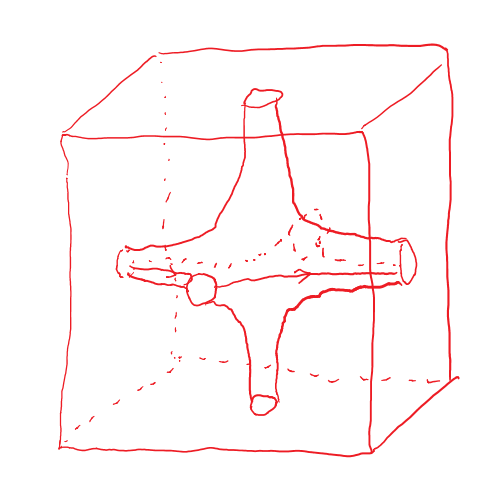
\includegraphics[scale=0.8]{100.png}}
		\\
		\textbf{B} in [110] direction:
		\\
		\centerline{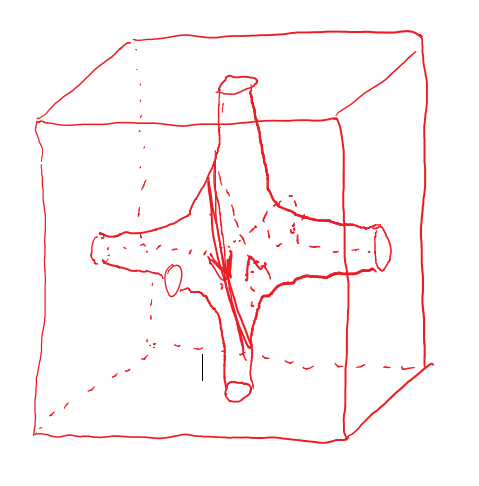
\includegraphics[scale=0.8]{110.png}}
		\\
		\textbf{B} in [111] direction:
		\\
		\centerline{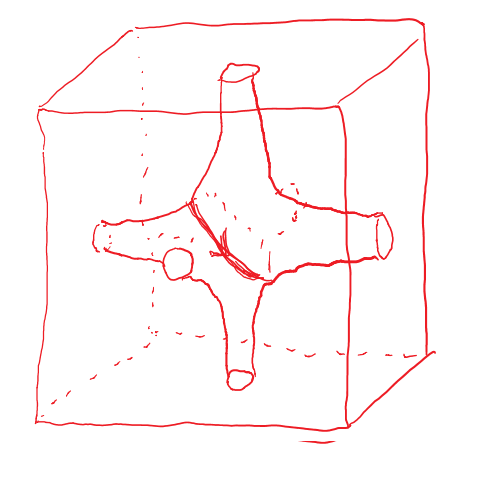
\includegraphics[scale=0.8]{111.png}}
		\\
	\end{homeworkProblem}


	\pagebreak

	\begin{homeworkProblem}
		\textbf{GaSb experimental data}\\
		
		The figure below is experimental data for an n-type GaSb (semiconductor) at $T=4.2K$. The Schubnikov-de Haas (SdH) trace ($\rho$ vs. $\frac{1}{\textbf{B}}$) is shown. The resistance ($\rho$) displays oscillatory behavior associated with the Landau levels piercing the Fermi surface.  The Hall resistance ($R_H$) is also provided.  
		\\
		\centerline{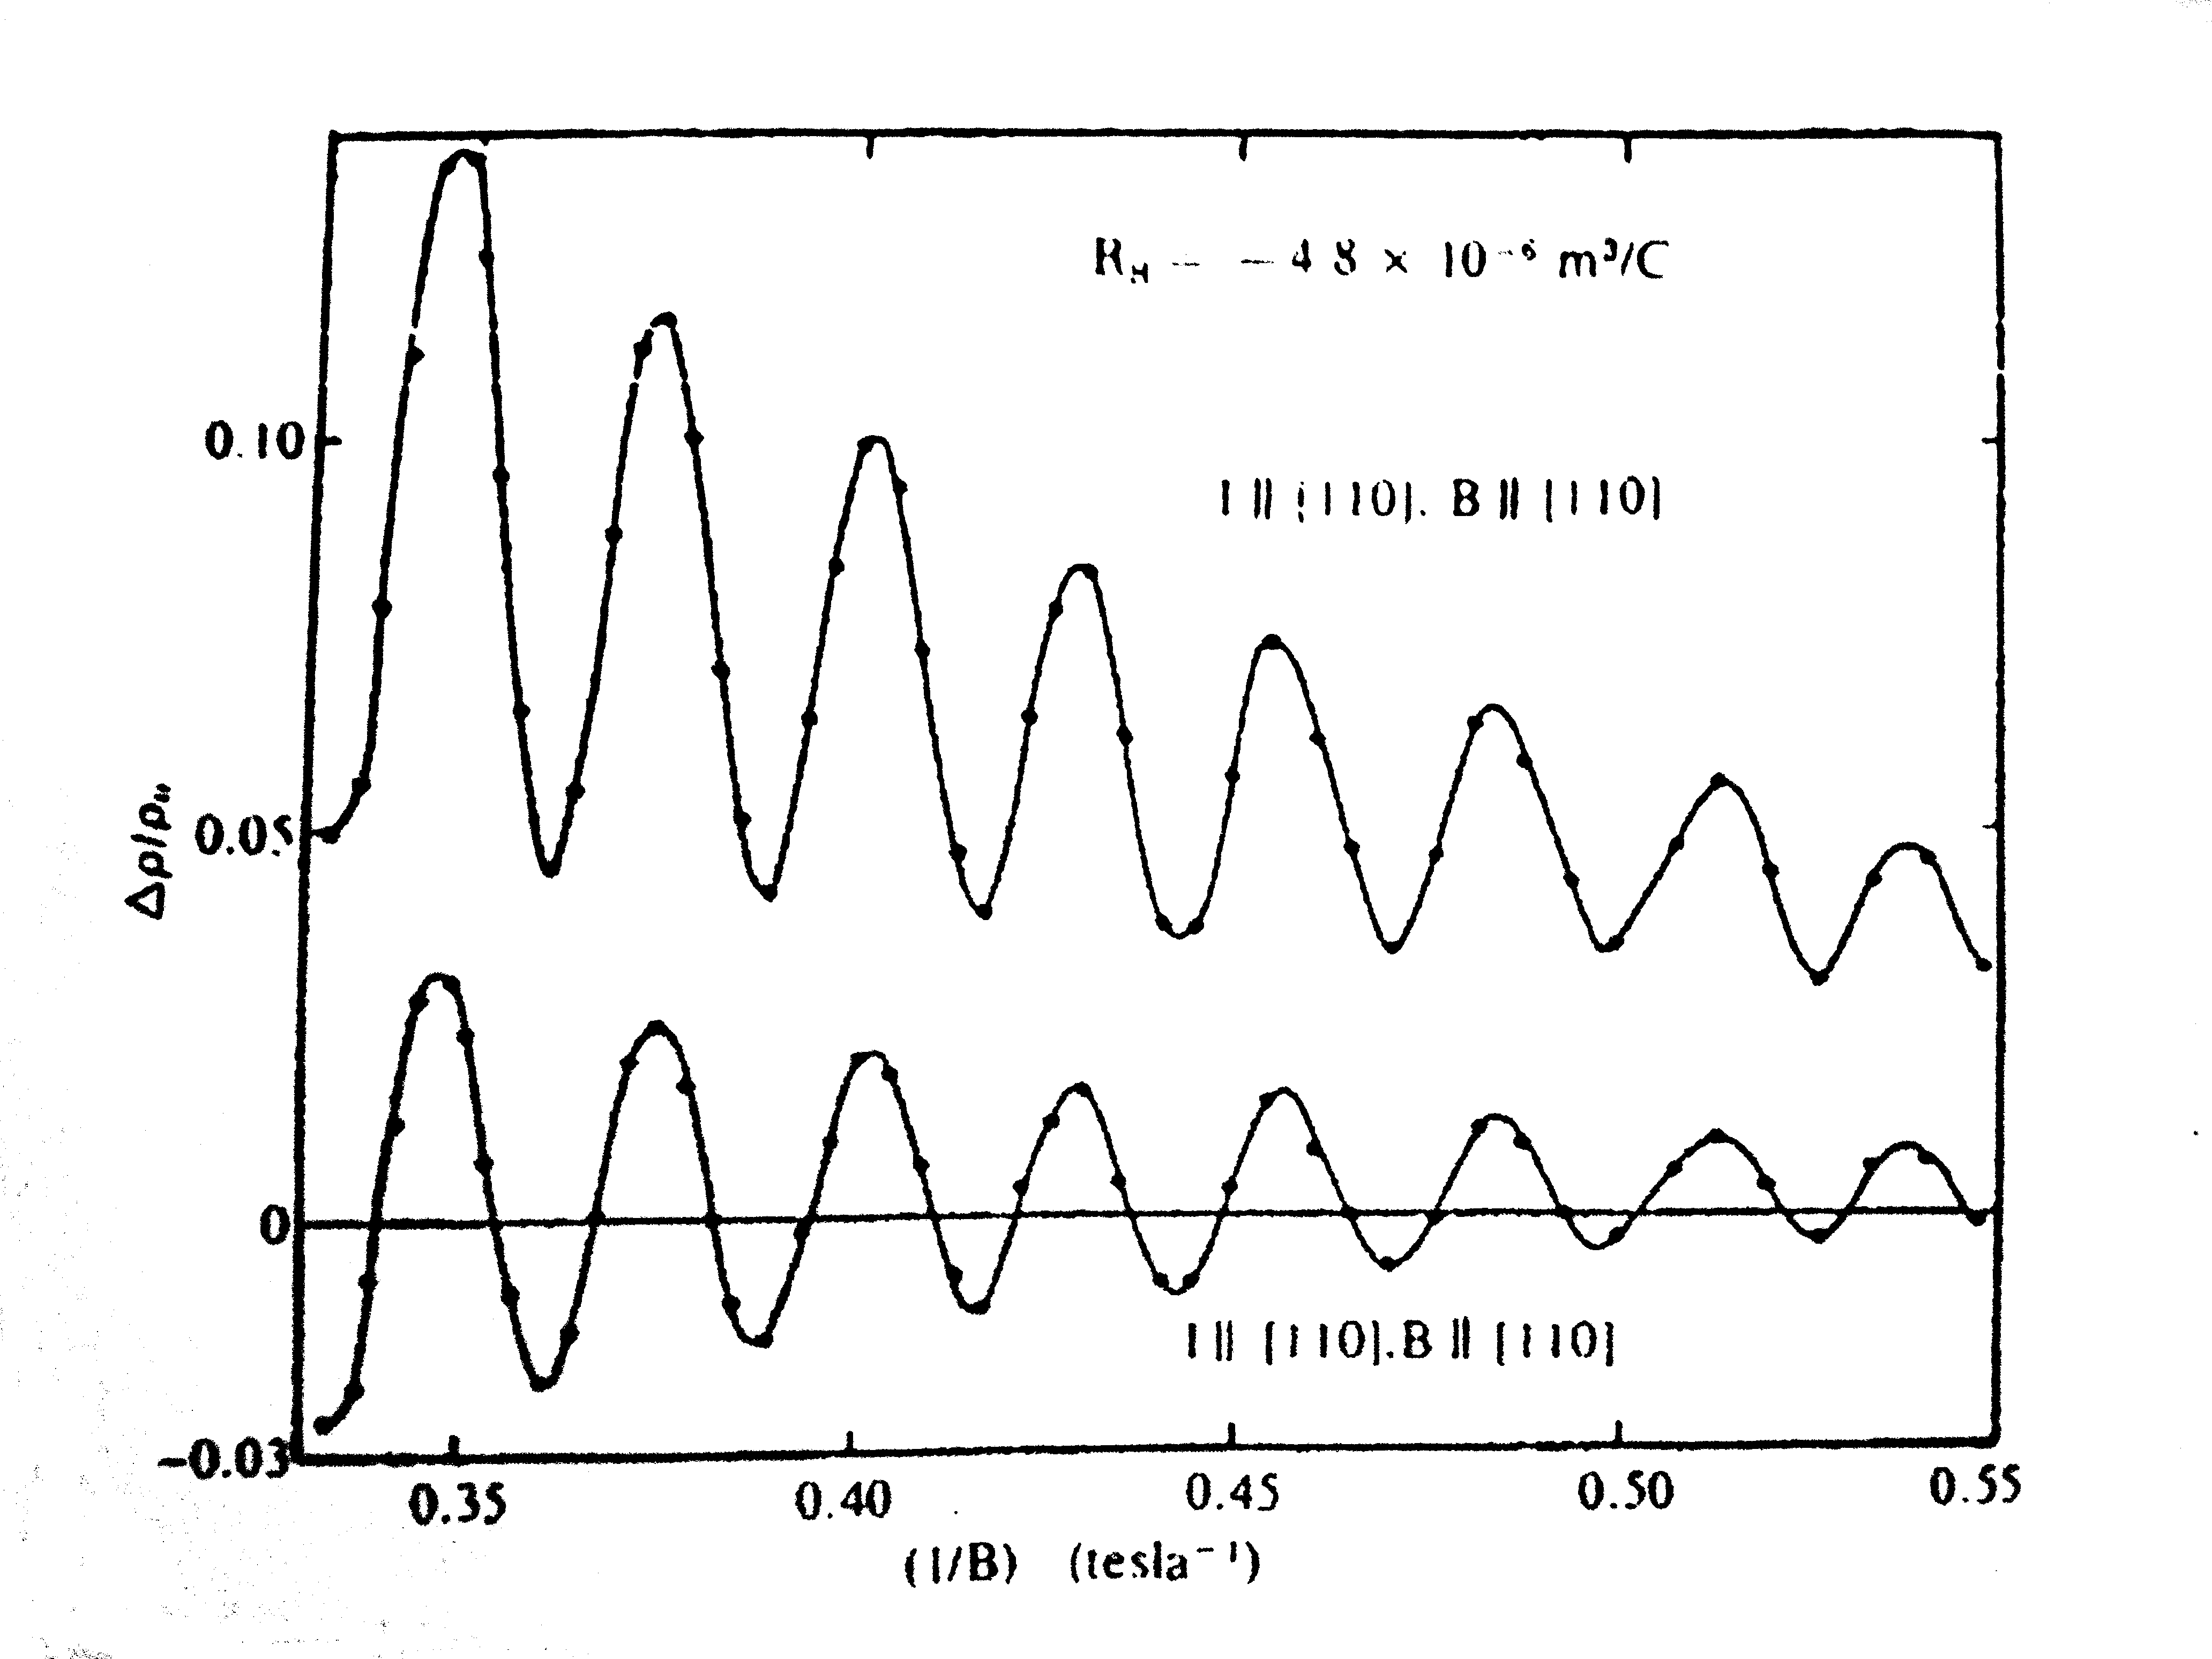
\includegraphics[scale=0.08]{20150402_011536.png}}
		\\
		Calculate the electron density from the SdH trace and see how it agrees with your calculation of the electron density from the Hall resistance.
\\
\\
		\textbf{Solution}\\
			
		The electron density is found by fitting the change in the magnetic field flux at the minima of each oscillation against the change in the resistance.  The following graph is created from the provided experimental data:
		\\
		\centerline{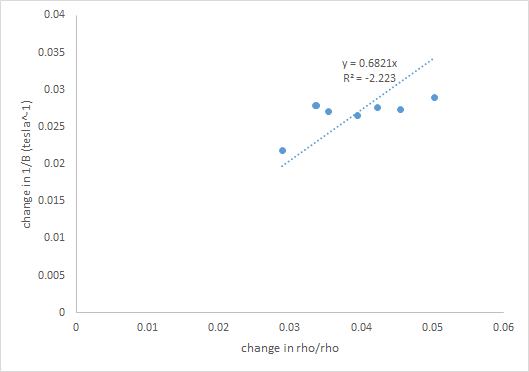
\includegraphics[scale=1]{exp_fit.png}}
		\\
		Using the following relation:
		\begin{equation*}
			n = \frac{2 e}{\Delta(\frac{1}{\textbf{B}})h}
		\end{equation*}
		We obtain that the electron density is:
		\begin{equation*}
			n = 700 \mu m^-2
		\end{equation*}

	\end{homeworkProblem}

	\pagebreak

	\begin{homeworkProblem}
		\textbf{Determining the band gap from temperature and intrinsic carrier concentration}\\
		
		The graph below displays the intrinsic carrier concentration for Ge, Si, and GaAs as a function of inverse temperature. 
		\\
		\centerline{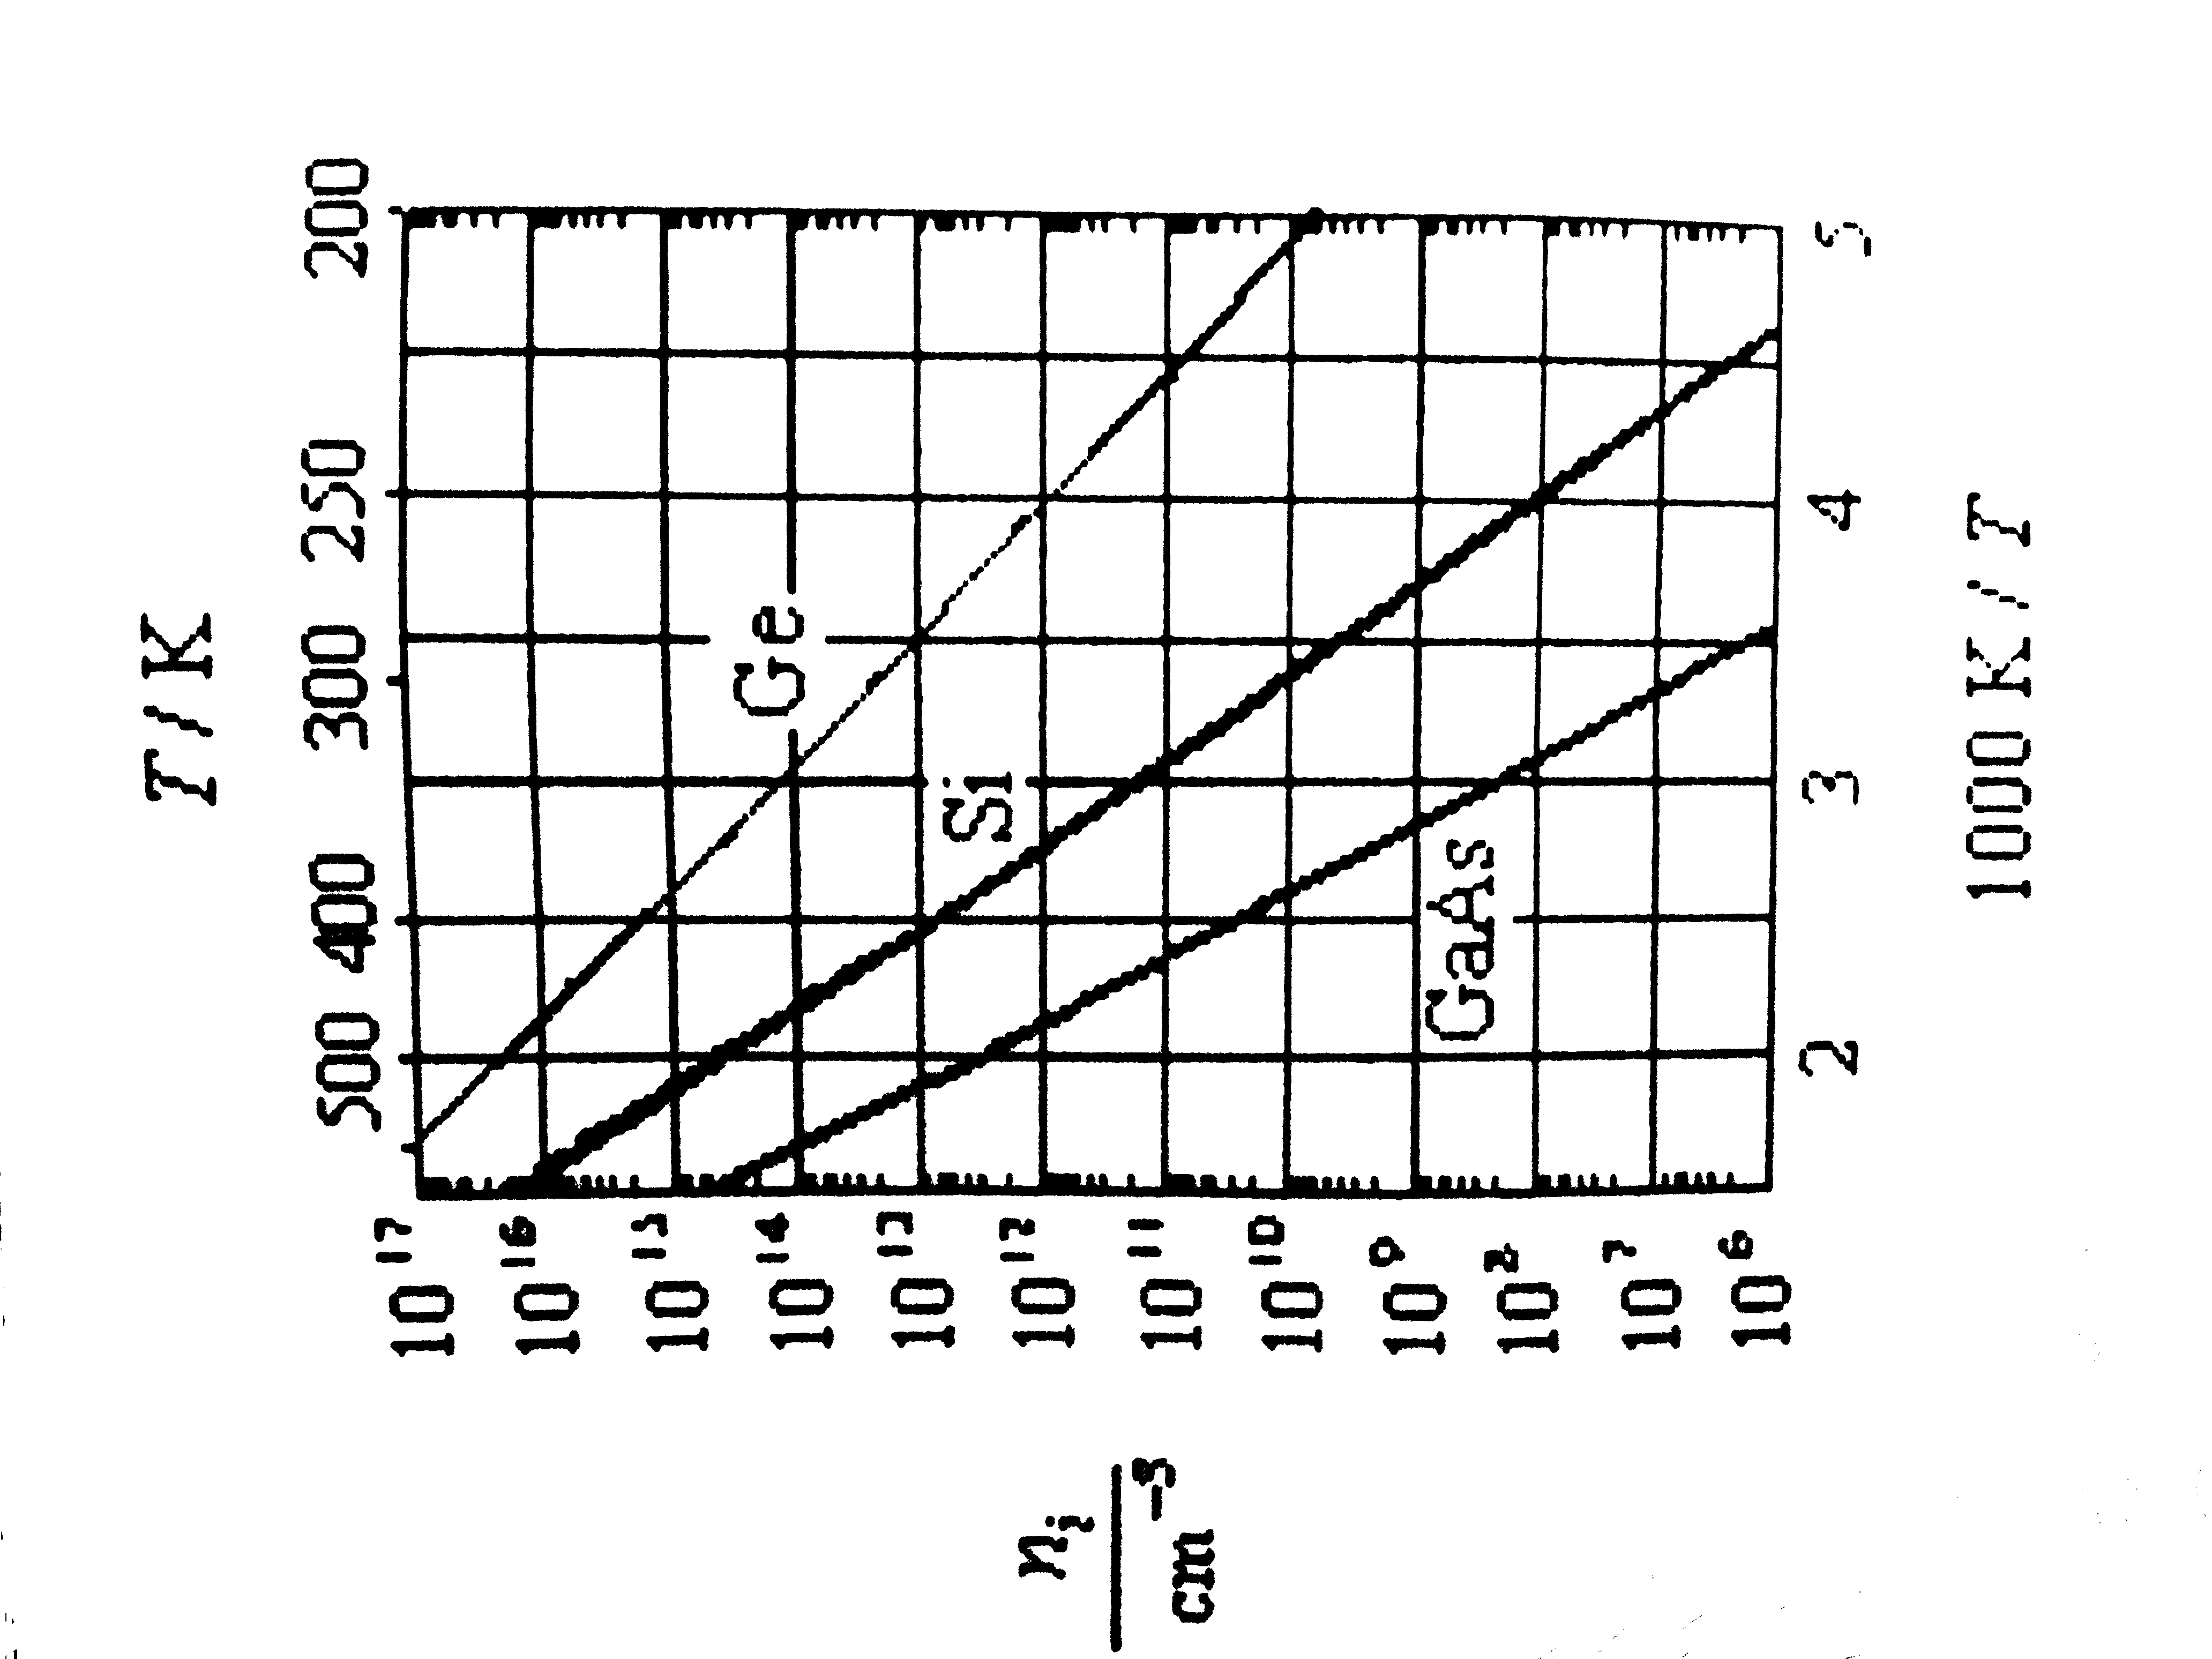
\includegraphics[scale=0.05,angle=-90]{20150402_011559.png}}
		\\
		Determine $E_g$ for each of the semiconductors using this graph.
		\\
		\\
		\textbf{Solution}\\
			
		The intrinsic carrier density is given by Chapter 8, Equation 45 in Kittel as:
		\begin{equation*}
			n_i = 2\Big(\frac{k_B T}{2\pi\hbar^2}\Big)^{\frac{3}{2}}(m_e m_h)^{\frac{3}{4}}e^{\frac{-E_g}{k_B T}}
		\end{equation*}
		The data in the graph can be fit using this equation and the band gap $E_g$ can be extracted.  Below is a graph of each fitting to the data.  
		\\
		\centerline{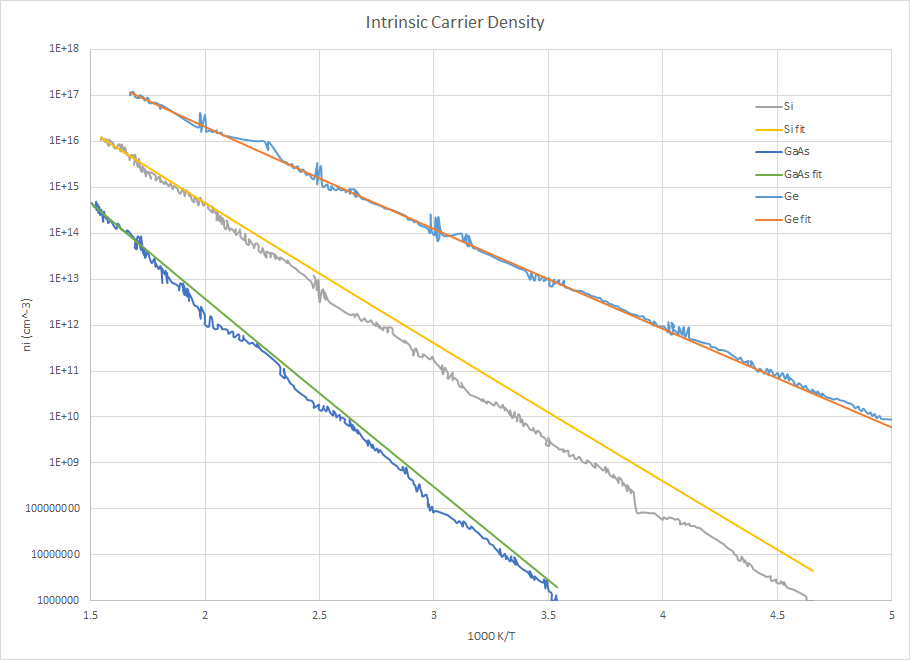
\includegraphics[scale=0.8]{Graph_fit.png}}
		\\
		The extracted band gaps are as follows:
		\begin{itemize}
			\item Germanium: 0.8 eV
			\item Silicon: 1.1 eV
			\item Gallium Arsenide: 1.5 eV
		\end{itemize}
	\end{homeworkProblem}
\end{document}
